\documentclass[conference]{IEEEtran}
\IEEEoverridecommandlockouts
% The preceding line is only needed to identify funding in the first footnote. If that is unneeded, please comment it out.
\usepackage{cite}
\usepackage{amsmath,amssymb,amsfonts}
\usepackage{algorithmic}
\usepackage{listings}
\usepackage{graphicx}
\usepackage{textcomp}
\usepackage{xcolor}
\def\BibTeX{{\rm B\kern-.05em{\sc i\kern-.025em b}\kern-.08em
    T\kern-.1667em\lower.7ex\hbox{E}\kern-.125emX}}
\begin{document}

\title{Implementing Minimum Error Rate Classifier\\
}

\author{\IEEEauthorblockN{Devopriya Tirtho}
\IEEEauthorblockN{16.02.04.033}
\IEEEauthorblockA{\textit{Department of Computer Science and Engineering} \\
\textit{Ahsanullah University of Science and Technology}\\
Dhaka, Bangladesh \\
}

}

\maketitle

\begin{abstract}
In \textbf{'Machine Learning'}, for predicting the accurate class of an unknown sample we need to visualize our training samples whether they are linearly separable or not. \textbf{'Minimum Error Rate'} classifier works with the help of bayes theory to generate the distribution of data points and then decide to predict the class of a data point.
\end{abstract}

\begin{IEEEkeywords}
Machine Learning,Minimum Error Rate Classifier, Gaussian Normal Distribution, Probability Density Function, Bayesian Decision Theory.
\end{IEEEkeywords}

\section{Introduction}
\textbf{Bayesian Decision Theory} is a probabilistic approach to find a particular pattern. The theory works with the quantisation of the trade-off between some cassification approaches by the help of probabilistic approach and the cost that accompany those approaches. Based on this theory, a classifier develops named \textbf{‘Minimum Error Rate Classifier'}. \textbf{Minimum Error Rate Classifier} is a classifier which tries to classify something by assuming the distribution of the thing with the help of \textbf{posterior probability} which consists of \textbf{likelihood probability} and \textbf{prior probability}. This type of classification method is called \textbf{generative approach}. Other machine learning approaches try to draw a fine line for classifying pattern whereas, this method try to understand the distribution of patterns.

\section{Task and Experimental Design}

There is a dataset named 'test' where all the datapoints are given. A row-matrix of $2$ elements represents the data. The given data works as the input data which has to be classified with the help of given prior probability information. The likelihood probability will be calculated with the help of given \textbf{mean} and \textbf{variance matrix}.\\
\begin{equation}
P(x|\omega 1)=N(\mu 1, \Sigma 1);\textrm{   }\\
\mu 1= \begin{bmatrix}
0 & 0 \\
\end{bmatrix}\\
\textrm{and }
\Sigma 1= \begin{bmatrix}
0.25 & 0.3 \\
0.3 & 1
\end{bmatrix}\\
\end{equation}
\begin{equation}
P(x|\omega 2)=N(\mu 2, \Sigma 2);\textrm{   }\\
\mu 2= \begin{bmatrix}
2 & 2 \\
\end{bmatrix}\\
\textrm{and }
\Sigma 2= \begin{bmatrix}
0.5 & 0.0 \\
0.0 & 0.5
\end{bmatrix}\\
\end{equation}
	$P(\omega 1)$= $0.5$\\
	$P(\omega 2)$= $0.5$\\
\begin{itemize}  
\item Our first task is to classify the sample points. For classification we use the \textbf{bayesian decision rule} which is :\\

\begin{equation}
P(\omega|x)=(P(x|\omega)*P(\omega))/P(x)\textrm{   }\\
\end{equation}
Here, the value of $likelihood\textrm{ }probability$ is unknown. The value of $likelihood\textrm{ }probability$ can be derived from the \textbf{Gaussian Normal Distribution's} formula. The formula is:\\
\begin{equation}
N_k(x_i|\mu_k,\Sigma_k)= \frac{e^{-0.5(x_i-\mu_k)^T\Sigma_k^{-1}(x_i-\mu_k)}}{\sqrt{(2\pi)^D|\Sigma_k|}}
\end{equation}
\item Secondly, we have to multiply the $prior$ value with the derived $likelihood$ value for each $\mu$ and $\Sigma$. Based on a decision rule, the classification occurs. The rule is:\\
\begin{equation}
P(x|\omega_1)*P(\omega_1)>P(x|\omega_2)*P(\omega_2)\textrm{   }\\
\end{equation}
$if \textrm{,   }true,$ class=$\omega_1$\\
$else \textrm{,   }$class=$\omega_2$\\
\item Thirdly, we have to plot the data in the graph as follows:\\
\begin{figure}[htbp]
\centerline{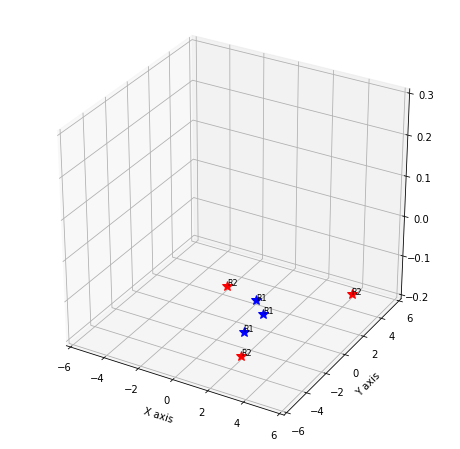
\includegraphics[scale=0.4673]{31.png}}
\caption{Datapoints of Class 1 and Class 2\\}
\label{fig}
\end{figure}


\item Then, we have to draw the probability density function and visualize with a contour graph as follows:\\
\begin{figure}[htb!]
\centerline{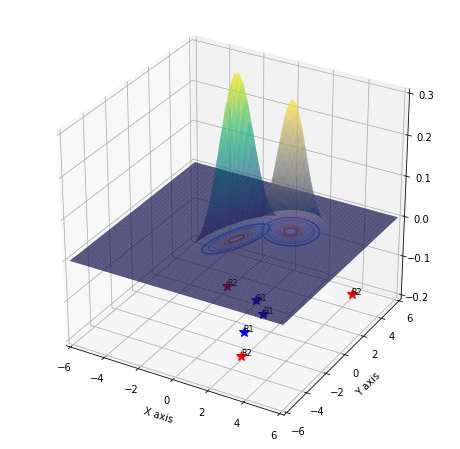
\includegraphics[scale=0.4673]{32.png}}
\caption{Visualization of Probability Density Function along with Its Contour\\}
\label{fig}
\end{figure}

\item Finally, we have to draw the \textbf{decision boundary} for the model. For drawing the decision boundary we have to find the $y-coordinate$ values for some $x-coordinate's$ values. I have taken a stream of data point from $-6$ to $6$ with equal difference of $0.5$ for the $sample\textrm{ }matrix$ and calculate the $y-coorcinates'$ value with the help of the following equation:\\ 
\begin{equation}
Y=\sqrt{\frac{\Sigma_1}{\Sigma_2}}e^{-\frac{(x-\mu_2)^T\Sigma_k^{-1}(x-\mu_2)}{2}+\frac{(x-\mu_1)^T\Sigma_k^{-1}(x-\mu_1)}{2}}\frac{\Theta}{1-\Theta}\\
\end{equation}
\begin{figure}[htb!]
\centerline{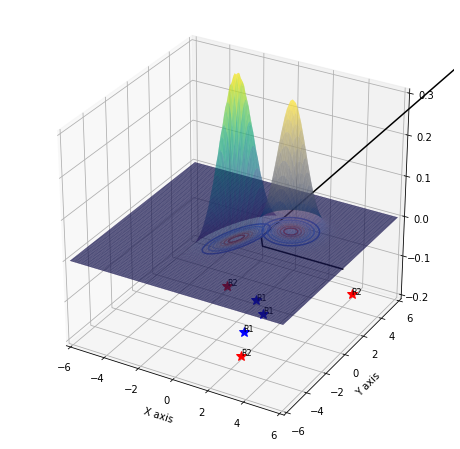
\includegraphics[scale=0.4673]{33.png}}
\caption{Drawing of Decision Boundary\\}
\label{fig}
\end{figure}
\\

\end{itemize}

\section{Result Analysis}
\begin{table}[htbp]
\caption{Table for Classification of Sample Data}
\begin{center}
\begin{tabular}{|c|c|c|}
\hline
\textbf{\textit{X1}}&\textbf{\textit{X2}}& \textbf{\textit{Class}} \\
\hline
\textbf{{1.0}}&\textbf{{1.0}}&   \textbf{{1}} \\
\hline
\textbf{{1.0}}&\textbf{{-1.0}}&   \textbf{{1}} \\
\hline
\textbf{{4.0}}&\textbf{{5.0}}&   \textbf{{2}} \\
\hline
\textbf{{-2.0}}&\textbf{{2.5}}&   \textbf{{2}} \\
\hline
\textbf{{0.0}}&\textbf{{2.0}}&   \textbf{{1}} \\
\hline
\textbf{{2.0}}&\textbf{{-3.0}}&   \textbf{{2}} \\
\hline
\end{tabular}
\label{tab1}
\end{center}
\end{table}

\section{Python Code}



\begin{lstlisting}
import pandas as pd 
import numpy as np 
import matplotlib.pyplot as plt

test_data = pd.read_csv('test.txt',
 sep=",", header=None) 
test_data.columns = ["x1", "y1"] 



#Declaring Parameters
prior1=0.5
prior2=0.5
mu1=np.array([0,0])
mu2=np.array([2,2])
sigma1=np.array([[0.25,0.3],[0.3,1]])
sigma2=np.array([[0.5,0],[0,0.5]])

print(mu1)
print(mu2)
print(sigma1)
print(sigma2)

det_sigma1= np.linalg.det(sigma1)
det_sigma2= np.linalg.det(sigma2)

print(det_sigma1)
print(det_sigma2)

from numpy.linalg import inv
inv_sigma1 = inv(sigma1)
inv_sigma2 = inv(sigma2)

print(inv_sigma1)
print(inv_sigma2)

b=test_data.shape
print(b[0])
RowNumber=b[0] 
PI = 3.14159

normal_dist_1=[]
normal_dist_2=[]

for i in range(0,RowNumber):
      test_datapoint=np.array
	([test_data.at[i,'x1'],
      test_data.at[i,'y1']])
      normal_dist_1.append
	((1/(2*PI*np.sqrt(det_sigma1)))
      *(np.exp(-0.5*(np.dot
	((test_datapoint - mu1).
transpose()
          , np.dot(inv_sigma1,
	(test_datapoint - mu1)))))))
	    normal_dist_2.append
	((1/(2*PI*np.sqrt(det_sigma2)))
          *(np.exp(-0.5*(np.dot
	((test_datapoint - mu2).
	transpose(),
           np.dot
	(inv_sigma2,
	(test_datapoint - mu2)))))))

posterior_1 = [i * prior1 for 
i in normal_dist_1]
posterior_2 = [i * prior2 for 
i in normal_dist_2]

print(posterior_1)
print(posterior_2)

#Testing Class
test_class=[]
for i in range(6):
  if (posterior_1[i]>posterior_2[i]):
    test_class.append(1)
  else:
    test_class.append(2)
test_data['class']=test_class

test_data

plot_data = pd.read_csv('plot.txt', 
sep=" ", header=None) 
plot_data.columns = ["x1", "y1"] 
plot_data

c=plot_data.shape 
print(c[0]) 
RowNumber=c[0] 
PI = 3.14159

coordinates=[]


for i in range(0,RowNumber):
    test_datapoint=np.array
    ([plot_data.at
    [i,'x1'],plot_data.at[i,'y1']])
    coordinates.append
    (np.sqrt(det_sigma1/det_sigma2)*
    (np.exp((-
    np.dot((test_datapoint - mu1).
    transpose(), 
    np.dot(inv_sigma1,
    (test_datapoint - mu1))))+
    (np.dot((test_datapoint - mu2).
    transpose()
    ,np.dot(inv_sigma2,
    (test_datapoint - mu2)))))))

Yd=np.array(coordinates)
X=plot_data['x1']
Xd=np.array(X)

import numpy as np
import matplotlib.pyplot as plt
from matplotlib import cm
from scipy.stats import multivariate_normal
from mpl_toolkits.mplot3d import Axes3D


x1=np.array(test_data['x1'])
y1=np.array(test_data['y1'])

#Parameters to set
mu_x = 0
variance_x = 3

mu_y = 0
variance_y = 15

#Create grid and multivariate normal
x = np.linspace(-6,6,100)
y = np.linspace(-6,6,100)
X, Y = np.meshgrid(x,y)
pos = np.empty(X.shape + (2,))
pos[:, :, 0] = X; pos[:, :, 1] = Y
rv = multivariate_norma
      l([0, 0], [[.25, .3], [.3, 1]])
rx = multivariate_norma
      l([2, 2], [[.5, 0], [0, .5]])
#Make a 3D plot

fig = plt.figure(figsize=(8,8))
ax= fig.add_subplot(111, projection="3d")
ax.plot_surface(X, Y, rv.pdf(pos), 
cmap="viridis",
 w=0.5, rstride=1, cstride=1, alpha=0.5)

ax.plot_surface(X, Y, rx.pdf(pos), 
cmap="cividis", 
w=0.5, rstride=1, cstride=1, alpha=0.5)

cset1 = ax.contour(X, Y, rv.pdf(pos), 
zdir='z', offset=0, cmap=cm.coolwarm)

cset2 = ax.contour(X, Y, rx.pdf(pos),
 zdir='z', offset=0, cmap=cm.coolwarm)

b=test_data.shape
print(b[0])
RowNumber=b[0] 

class_1_x=[]
class_1_y=[]
class_2_x=[]
class_2_y=[]
for i in range(0,RowNumber):
  if (test_data.at[i,'class']==1):

    class_1_x.append
	(test_data.at[i,'x1'])	
    class_1_y.append
	(test_data.at[i,'y1'])

  else:
    class_2_x.append
	(test_data.at[i,'x1'])
    class_2_y.append
	(test_data.at[i,'y1'])


class_1_x=np.array(class_1_x)
class_1_y=np.array(class_1_y)
class_2_x=np.array(class_2_x)
class_2_y=np.array(class_2_y)

ax.plot3D(class_1_x,class_1_y,-0.2,
'b*', 
markersize=10,label='Train Class 1')
ax.plot3D(class_2_x,class_2_y,-0.2,
 'r*', 
markersize=10,label='Train Class 2')


ax.text(class_1_x[0], class_1_y[0],
-0.2, "R1", size=8,color='k') 
ax.text(class_1_x[1], class_1_y[1],
-0.2, "R1", size=8, color='k') 
ax.text(class_1_x[2], class_1_y[2],
-0.2, "R1", size=8, color='k') 
ax.text(class_2_x[0], class_2_y[0],
-0.2, "R2", size=8, color='k') 
ax.text(class_2_x[1], class_2_y[1],
-0.2, "R2", size=8,color='k') 
ax.text(class_2_x[2], class_2_y[2],
-0.2, "R2", size=8, color='k') 

ax.plot(Xd,Yd,0,color='black')
ax.set_xlim(-6, 6)
ax.set_ylim(-6, 6)
ax.set_zlim(-0.2, 0.3)

ax.set_xlabel('X axis')
ax.set_ylabel('Y axis')
#ax.set_zlabel('Probability Density')
plt.show()
\end{lstlisting}


\section{Conclusion}

\textbf{‘Minimum Error Rate Classifier’} is a simple classification technique which uses probabilistic method to classify sample points. This algorithm works with the help of \textbf{Gaussian normal distribution} and assumes the distribution of a pattern. From the distribution it predicts the class of data.




\end{document}
